% This is LLNCS.DEM the demonstration file of
% the LaTeX macro package from Springer-Verlag
% for Lecture Notes in Computer Science,
% version 2.4 for LaTeX2e as of 16. April 2010
%
\documentclass{llncs}

\usepackage{makeidx}  % allows for indexgeneration
\usepackage{comment} % multi-line comments
\usepackage{graphicx} % necessary for inclusion of .eps for figures
\usepackage{algpseudocode}
\usepackage{amsmath}
\usepackage{times}
\usepackage{setspace}
\usepackage{acronym}
\usepackage{caption}
\usepackage{adjustbox}

\graphicspath{ {./drawings/} {./plots/} }
\begin{document}
%
\frontmatter          % for the preliminaries
%
\pagestyle{headings}  % switches on printing of running heads
%\addtocmark{Hamiltonian Mechanics} % additional mark in the TOC
%
\mainmatter
\title{Application of Congestion Notifications in a Cyber-Physical System}
%
\titlerunning{Application of Congestion Notifications}  % abbreviated title (for running head)
%                                     also used for the TOC unless
%                                     \toctitle is used
%
\author{Stephen Jackson \and Dr. Bruce McMillin }
%
\authorrunning{Stephen Jackson et al.} % abbreviated author list (for running head)
%
%%%% list of authors for the TOC (use if author list has to be modified)
%\tocauthor{Ivar Ekeland, Roger Temam, Jeffrey Dean, David Grove,
%Craig Chambers, Kim B. Bruce, and Elisa Bertino}
%
\institute{Missouri University of Science \& Technology, Rolla, MO 65409, USA,\\
\email{\{scj7t4,ff\}@mst.edu}}

\maketitle              % typeset the title of the contribution

\newacro{FREEDM}{Future Renewable Electric Energy Delivery and Management}
\newacro{DGI}{Distributed Grid Intelligence}
\newacro{CPS}{cyber-physical system} 
\newacro{AYC}{Are You Coordinator}
\newacro{AYT}{Are You There}
\newacro{RED}{Random Early Detection}
\newacro{NS3}[NS-3]{Network Simulator 3}
\newacro{ECN}{Explicit Congestion Notification}
\newacro{VANET}{Vehicular Ad Hoc Networks}
\newacro{EWMA}{Exponentially Weighted Moving Average}
\newacro{CDF}{Cumulative Distribution Function}


\begin{abstract}

\begin{abstract}
Cyber-physical systems (CPS) are an attractive option for future development of
critical infrastructure systems. By supplementing the traditional physical
network with cyber control, the performance and reliability of the system
can be increased. In some of these networks, distributing the cyber control
offers increased redundancy and availability during fault conditions. However,
there are very few works which study the effects of cyber faults on a 
distributed cyber-physical system. These are of a particular interest in the smart grid
environment where outages and failures are very costly. By examining the
behavior of a distributed system under fault scenarios, the overall robustness
of the system can be improved by planning characteristics and responses to
faults that allow the system to continue operating in difficult circumstances.

This work examines the consequences of network unreliability on a core part of the
 Distributed Grid Intelligence (DGI) for the FREEDM (Future Renewable Electric 
Energy Delivery and Management) Project. By applying different rates of packet
loss in specific configurations to the communication stack of the software and
observe the behavior of a critical component (Group Management) under those
conditions. These components identify the amount of time spent in a group,
working, as a function of the network reliability. Given this one can parameterize
the amount of messages that are lost and thus the number of failed physical actuations.
Knowing this and the physical characteristics of the system, one can tune the amount
of time between reconfiguration in order to prevent the number of failed physical
changes from causing the system to become unstable. Using this, we can develop
methods and guarantees to protect the operation of a CPS.
\end{abstract}

\keywords{smart-grid, cyber-physical systems, real-time systems, distributed systems, network congestion}
\end{abstract}

% Introduce the contents of the paper and what will be presented
\chapter{Introduction}

The design of stochastic models of distributed systems has a long history as a challenging area of interest.
Models of distributed systems have to deal with a number of factors.
These factors include the various types of failure the system could experience, a lack of tightly synchronized execution, and a large complex state space when there are a high number of agents\cite{DISTRIBUTED}\cite{distributed-challenges}. 
However, the concept of distributed systems plays a central role in many of the future visions for how critical infrastructure will operate.
These critical infrastructures are physical networks whose operation are so vital that if those networks failed to operate correctly it would be highly detrimental to the population that rely on those systems.
\ac{CPS} are the integration of computational systems with physical networks.
Computational systems already play a critical role in most critical infrastructures, and as demands for security features, such as accessibility, increase distributed systems are becoming an increasingly favorable choice for the computational needs for these systems\cite{SMARTGRIDBENEFITS}.

The \ac{FREEDM} center\cite{FREEDM}, an NSF funded ERC envisions a future power-grid where widely distributed renewable power generation and storage is closely coupled with a distributed system that facilitates the dispatch of power across those areas.
Other systems like \ac{VANET}\cite{CARS1}\cite{CARS2}\cite{vanet-congestion} and air traffic control systems\cite{AIRTRAFFIC1}\cite{AIRTRAFFIC2} also propose similar control systems where many computers must cooperate to ensure both smooth operation and the safety of the people using those systems.
As a consequence, ensuring that the computer systems that control those infrastructures behave correctly during fault conditions is critical, especially when those computer systems rely on their interaction with other computers to operate.

A robust \ac{CPS} should be able to survive and adapt to communication network outages in both the physical and cyber domains.
When one of these outages occurs, the physical or cyber components must take corrective action to allow the rest of the system to continue operating normally.
Additionally, processes may need to react to the state change of some other process.
Managing and detecting when other processes have failed is commonly handled by a leader election algorithm and failure detector.

In a smart-grid system, misbehavior during fault conditions could lead to critical failures such as a blackout or voltage collapse. In a \ac{VANET} or air traffic control system, vehicles could collide, injuring passengers or destroying property. Additionally, since these systems are a part of critical infrastructure, protecting them from malicious entities is an important consideration.

This work was motivated by observations on the effects of lost messages on the group management module of the \ac{DGI} used by the \ac{FREEDM} smart-grid project.
These original observations confirmed the need to explore more well defined models for the behaviors of \ac{CPS} in order for them to better serve the people that use them.

We present a framework for reasoning about inferable state in the context of a distributed system. To do this, we exploit existing work in the field of information flow security. Information flow security has been used to reason about how attacks like STUXNET can manipulate operators beliefs while disrupting a system\cite{STUXNET}. In particular, these approaches reason about how the operator in a STUXNET attack has no avenue to verify the reports from a compromised computing device. Using existing modal logic frameworks and using information flow security models\cite{Howser2012}\cite{STUXNET}\cite{Howser2013}, one can formally reason about where information that is not normally known to a domain can be inferred.

We will show in this work that in a system with the correct information flows, an agent in a distributed system can infer the state of other agents in the system. With this information, that agent can then construct a reasonable model of the system to determine if the current behavior could lead to an undesirable situation with either the cyber or physical network.

Using this framework we present a leader election algorithm that can be modeled with a Markov chain for a known omission fault\cite{OMISSIONFAILURES} rate.
The presented algorithm maintains the Markov property for the observations of the leader despite omission faults.
This approach to considering how a distributed system interacts during a fault condition allows for the creation of new techniques for managing a fault scenario in cyber-physical systems.
In the context of \ac{FREEDM}, these models produce expectations of how much time the DGI will be able to spend coordinating and doing useful work.
Using these measures, the behavior of the control system for the physical devices can be adjusted to prevent faults, like blackouts and voltage collapse, in the physical network.

We also propose using existing schemes to detect communication network congestion and inform processes in a \ac{CPS} of impending congestion.
Processes act on this information to change their behavior in anticipation of message delays or loss.
This behavior allows them to harden themselves against the congestion, and allows them to continue operating as normally as possible during the congestion.
This technique involves changing the behavior of both the leader election\cite{INVITATIONELECTION} and physical device management algorithm during congestion.

To accomplish this, we extend existing networking concepts of \ac{RED}, \ac{ECN}\cite{RFCECN}, and ICMP source quench\cite{RFCSOURCEQUENCH}.
When a network device detects congestion, it notifies processes that the network is experiencing congestion and they should react appropriately.
We demonstrate an implementation of the \ac{FREEDM} \ac{DGI} in a \ac{NS3} simulation environment\cite{NS3} with our congestion detection feature.
The \ac{DGI} operates normally until the simulation introduces a traffic flow that congests the network devices in the simulation.
After congestion has been identified by the \ac{RED} queuing algorithm, the \ac{DGI} are informed. %via UDP multicast.
When the congestion notifications are introduced, the \ac{DGI} maintains configurations which they would normally be unable to maintain during congestion.
Additionally, we show a greater amount of work can be done without the work causing unstable power settings to be applied.


\chapter{Background}

\section{Distributed Systems}

Distributed systems are a computing paradigm characterized by independence of computational units and no universal clock.
Components in a distributed system may not directly share computational resources or memory.
Instead, computers in a distributed system typically interact through a message passing interface.

As a result, distributed computing is a challenging area of research.
In a distributed system, because processes do not share a universal clock, the ordering of messages and events needed to be carefully considered to ensure correct operation of the system.
Additionally, when individual components fail, determining which components fail and how they affect the system as a whole is also difficult in a distributed system.
Different types of failures can cause different kinds of information to be withheld or changed, disrupting those processes.

\section{Execution And Communication Models}

We consider a distributed system where no processes in the system share an address space.
All processes must use a message passing interface to communicate with other processes to exchange information.
As a result of the complexities of distributed systems, various execution models have been developed to define how the execution of a distributed system proceeds.
Different execution models affect how easy it is to reason about the system's execution, the types of algorithms the system can execute, and how complicated they are to implement.

\subsection{Communication Channels}
We describe the avenues of communication between processes as channels.
A channel is classified as reliable if it meets three axioms:

\begin{axm}
    \label{axm:reliable-channel-sender}
    Every message sent by a sender is received by a receiver and every received message was sent by a sender in the system. \cite{DISTRIBUTED}
\end{axm}

\begin{axm}
    \label{axm:reliable-channel-delay}
    Every message has an arbitrary but not infinite propagation delay.\cite{DISTRIBUTED}
\end{axm}

\begin{axm}
    \label{axm:reliable-channel-fifo}
    Every channel is a \ac{FIFO} channel. If process $P$ sends a messages $x$ and $y$ to $Q$ (in that order) then $Q$ receives the messages in order ($x$ then $y$).\cite{DISTRIBUTED}
\end{axm}

Reliable channels are often referred to as synchronous channels.
However, in our system, channels are not assumed to be perfectly reliable.
Instead, we respect Axioms \ref{axm:reliable-channel-fifo} \& \ref{axm:reliable-channel-fifo}, partially fulfill Axiom \ref{axm:reliable-channel-sender}, and disregard Axiom \ref{axm:reliable-channel-delay}.
Therefore, we assume the following about communication channels in our systems (replacing Axiom \ref{axm:reliable-channel-sender}):

\begin{axm}
    Every message received by a receiver was sent by a sender in the system.
\end{axm}

Without the constrained propagation delay from \ref{axm:reliable-channel-delay}, this type of communication channel is typically referred to as an asynchronous channel.

The communication model can be synchronous or asynchronous.
In the synchronous communication model, processes can only send a message when the receiving process is ready to receive it.
Algorithmically, sending in a synchronous model is usually considered a ``blocking'' operation, meaning, once a process tries to send a message, it cannot proceed until the message is received.
In this work, communication is asynchronous: a process does not wait for the successful delivery of a message, typically referred to as a non-blocking send.

\subsection{Clocks}
Clocks are considered synchronized if every clock in the system reads the same time.
Since it is impossible for independent clocks to tick at the same rate, weak synchronization is used to describe when clocks in the system have an upper bound on drift rate from each other.

\subsection{Execution}
In a system with synchronous processes, processes execute in lockstep.
At each step, a process executes its next available action.
Synchronous execution requires the strong organization of the processes executing the algorithm.
The systems presented rely on partially synchronous execution by processes.
In the partially synchronous model, execution proceeds in rounds or phases.
The start of each round or phase is synchronized between processes, using a synchronized clock.

\section{Faults, Failures, and Errors}

Processes can encounter incorrect behavior or issues during execution.
Errors, faults, and failures describe the severity and consequence of the issue.

\begin{pdef}
An error is a difference between what is considered ``correct'' output for a given component, and the actual output: an incorrect result.
\end{pdef}

\begin{pdef}
A fault is the manifestation of an error in software or an incident where an incorrect step, or data definition is performed in a computer program.
\end{pdef}

\begin{pdef}
Failure is the inability of a component or system to perform its required function or within its specified limits.
\end{pdef}

\subsection{Crash or Fail-Stop Failure}

A crash failure or its more generalized form, a fail-stop failure, describes a failure in which a process stops executing.
In general, it is considered to be an irreversible failure, since a process typically does not resume from a crashed state.
There is a special category of crash failures, called napping failures, where a process will appear to have crashed for a finite amount of time before resuming normal operation.
Crash failures are impossible to detect with absolute certainty in an asynchronous system.
Processes can be suspected by other processes through the use of challenge/response messages or heartbeat messages that allow a process to prove that it has not crashed yet.
A system that can handle a crash failure is implied to be able to handle a fail-stop failure.\cite{DISTRIBUTED}

The fail-stop failure has three properties \cite{DISTRIBUTED}:

\begin{enumerate}
\item When a failure occurs the program execution is stopped.
\item A process can detect when another fail-stop process has failed.
\item Volatile storage is lost when the fail-stop process is stopped.
\end{enumerate}

\subsection{Omission Failure}

An omission fault\cite{OMISSIONFAILURES} occurs when a message is never received by the intended recipient.
Omission faults can occur when the communication medium is unavailable or when the latency of message exceeds a timeout for its expected delivery.
Protocols like TCP do not tolerate omission failures: a packet is resent until it is acknowledged by the receiver.
If the acknowledgment never comes, the connection is closed.
As a contrast, UDP assumes that any datagram could be lost, and it is the responsibility of the programmer to handle missing datagrams appropriately.
An omission failure can have the same observable effects as a napping failure in some situations.\cite{DISTRIBUTED}


\subsection{Failure Detectors}

Failure detectors\cite{FAILUREDETECTORS} (Sometimes referred to as unreliable failure detectors) are a special class of processes in a distributed system used to detect other failed processes.
Distributed systems use failure detection to identify failed processes for leader election routines.
Because it isn't possible to directly detect a failed process in an asynchronous system, there has been a wide breadth of work related to different classifications of failure detectors, with different properties.
Some of the properties include\cite{FAILUREDETECTORS}:

\begin{itemize}
    \item Strong Completeness - Every faulty process is eventually suspected by
        every other working process.
    \item Weak Completeness - Every faulty process is eventually suspected by 
        some other working process.
    \item Strong Accuracy - No process is suspected before it fails.
    \item Weak Accuracy - There exists some process is never suspected of failure.
    \item Eventual Strong Accuracy - There is an initial period where strong accuracy is not kept. Eventually, working processes are identified as such, and are not suspected unless they actually fail.
    \item Eventual Weak Accuracy - There is an initial period where weak accuracy is not kept. Eventually, working processes are identified as such, and there is some process that is never suspected of failing again.
\end{itemize} 

One class of failure detectors, Omega class Failure detectors, are particularly interesting because of \cite{LEADERELECTIONEVAL}. An eventual weak failure (weak completeness and eventual weak accuracy) detector is the weakest detector which can still solve consensus. It is denoted several ways in various works including $\diamond \mathcal{W}$ \cite{FAILUREDETECTORS}, $\mathcal{W}$ \cite{WEAKESTFAILURE1} \cite{WEAKESTFAILURE2} and $\Omega$ (Omega) \cite{LEADERELECTIONEVAL}.


\subsection{Byzantine Fault}

Byzantine fault, causes processes in the distributed system send information that is incorrect or misleading to other processes.
Constraints for detecting processing that exhibit Byzantine behavior is a famous result in distributed systems.\cite{byzantine-generals}

\section{Probability}

Several concepts are useful for reasoning about the stochastic properties of a distributed system.
The expected value represents the long-term average output of a probability distribution.

\begin{equation}E[X] = x_1 p_1 + x_2 p_2 + ... + x_k p_k \end{equation}

\nomenclature{$E[X]$}{Expected value of a random variable.}
Conceptually, the expected value is the weighted average of the outcomes of some stochastic system.

\begin{pdef}
Availability is the probability a system or component is operational and accessible when required for use, denoted $A$.
\end{pdef}

\begin{equation}A = \frac{E[uptime]}{E[uptime]+E[downtime]}\end{equation}
\nomenclature{$A$}{Availability of a component.}

\begin{pdef}
Reliability is the ability of a system or component, in specified conditions, to be able to perform its required functions for a specified period.
\end{pdef}

\begin{equation}R(t) = \Pr(T > t) = \int_t^{\infty} f(x) dx\end{equation}
\nomenclature{$R(t)$}{Reliability of a component.}

Where $R(t)$ is the probability that the system or component functions up until at least time $t$ and $f(x)$ is the probability density function for the component's survival.
Unfortunately, there is a clash of the term for reliability in distributed systems and reliability analysis.
We try to constrain the discussion about reliability in the distributed systems sense to communication channels.

\section{Markov Models}

%When Markov chains work to model a system.
%Something about order of Markov chain.
%State what a Markov chain and the properties of the Markov chain.
%State what states mean.
%State what transition probabilities mean. State what ergodicity is. State what stationarity is. State how we generate the sequence of states.

\nomenclature{$X$}{A random variable, or the set of states for a Markov chain}%
A Markov chain is a finite set of states $X=\{x_1, x_2, ..., x_n\}$ and probabilistic transitions between those states.
States in a Markov chain are mutually exclusive.
In a Markov chain, when a system is some state $x_i$ it has some probability of transitioning to some other state $x_j$ at the next time-step.
A Markov chain is a first order chain if the probability of transitioning from $i$ to $j$ does not depend on the history of transitions that lead to state $i$.
First order chains are described as having a memoryless or Markov property.
The Markov property formalizes the independence of the next state from the history of previous states.
The Markov property describes a Markov chain as a sequence of random variables $X_{1}, X_{2}, X_{3}, ...$ and states the value of $X_{n+1}$ only depends $X_{n}$: \cite{MARKOV3}

\begin{align} \Pr(X_{n+1}&=x\mid X_1=x_1, X_2=x_2, \ldots, X_n=x_n)
\nonumber \\ &= \Pr(X_{n+1}=x\mid X_n=x_n). \end{align}

An ergodic Markov chain is a chain where it is possible, in some finite number of steps, to go from any state to any other state.
A stationary, or time homogeneous, Markov chain is one where the transition probabilities do not change over time.
In a stationary Markov chain, the $n$th visit to a state is indistinguishable from the $n+1$th visit to a state.

\subsection{Discrete Time Markov Chain}

\nomenclature{$P$}{Transition probability matrix of a discrete time Markov chain.}
A \ac{DTMC} is one where the transitions between states happen at discrete time steps.
A \ac{DTMC} with $m$ states can be represented by a $m\times m$ matrix.
For simplicity when creating the model, matrices in this work are 1-indexed.
In a matrix $P$, the value of $P_{ij}$ represents the probability of the transition from $x_i$ to $x_j$.
The matrix is row stochastic, meaning the sum of each row in the matrix is equal to one:

\begin{equation} \sum_{i=1}^{m} P_{ij} = 1. \end{equation}

A useful companion to the transition matrix is a state distribution vector.
While the transition matrix describes how a system will transition between states, the state distribution vector describes the probability of observing a given state.

\begin{pdef}
A state distribution vector is an $m$-dimensional vector composed of probability of observing each state in the system at a given instant:
\[ [P_{1} \quad P_{2} \quad \ldots \quad P_{m} ] \]
Where $P_{i}$ corresponds to the probability of observing state $x_i$.
\end{pdef}

A \ac{DTMC} is a suitable model for a memoryless random process with a finite number states which is observed at fixed time intervals.
By utilizing a Markov chain, a variety of statistical analyses can be performed on the modeled system.
For example, a Markov chain with the stationary and ergodic properties can be analyzed for its steady state probabilities.
The steady state is a state distribution vector that describes the probability a random observation of a long-running process will observe some state $x_i$.
The steady state probability distribution vector can by found via a system of equations: \cite{MARKOV3}

\begin{align}
0\leq\pi_j\leq1.0 \\
\sum_{j = 1}^{m}\pi_j = 1.0 \\
\pi_j = \sum_{i=1}^{m} \pi_i p_{ij}
\end{align}

The computation of the steady state will be noted as $Steady()$.
A Markov chain can also be used to predict what state a process will be in at some point in the future.
Given an initial state and a number of time-steps, a matrix operation will yield the likelihood of the process being in each state after the time interval has passed.
The mean passage time, a measure of how many time-steps will pass before a process returns or arrives in some state, can also be calculated.

We model a leader election algorithm with a closed form representation of the behavior of the algorithm.
The closed form representation is a profile Markov chain (noted as $P$) and will be validated against a chain generated from execution of the algorithm.
The chain constructed from sampled data is known as a test chain (noted as $T$).
\nomenclature{$T$}{Test chain. A Markov chain sampled from a system.}

\subsection{Continuous Time Markov Chain}

Transitions in a \ac{CTMC} depend on the amount of time spent in a given state.
Let $X(s) = x_i$ indicate the model is in state $x_i$ at time $s$.
If the model is time homogeneous, then the probability of transitioning to state $x_j$ only depends on the time spent in the current state ($t$).

\begin{equation}
    \Pr\{ X(s+t)=x_j | X(s) = x_i \} = \Pr\{ X(t)=x_j | X(0) = x_i \}
\end{equation}

Each transition has some expected value or holding time which describes the amount of time before a transition occurs.
The \ac{pdf} of the exponential distribution can be written as: \cite{MARKOV1}

\begin{equation}
f(x;\lambda) = \begin{cases}
\lambda e^{-\lambda x} & x \ge 0 \\
0 & x < 0
\end{cases}
\end{equation}

As a result, the expected or mean value of an exponential distribution is a function of the parameter $\lambda$: \cite{MARKOV1}

\begin{equation}
\mathrm{E}[X] = \frac{1}{\lambda}. \!
\end{equation}

When there are multiple possible transitions from a state, each with their own expected transition time, the expected amount of time in the state is: \cite{MARKOV2}
\begin{equation}
\sum \lambda(x,y) = \sum \lambda p_{x,y} = \lambda(x)
\end{equation}
where $\lambda(x,y)$ is the expected amount of time before state $x$ transitions to state $y$.
The expected time in a state ($\lambda(x)$) is related to the expected time for an individual transition ($\lambda(x,y)$) by a probability $p_{x,y}$.
Each transition contributes to an expected amount of time in the state.

\subsection{Hidden Markov Model}

\begin{figure}
	\centering
	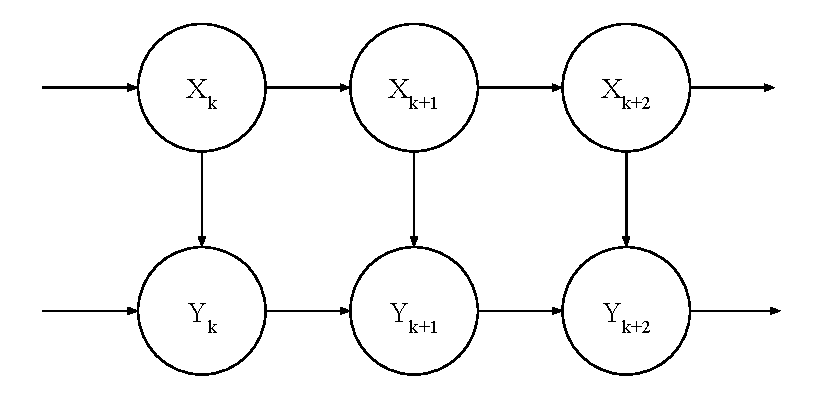
\includegraphics[width=0.75\textwidth]{hiddenmarkovmodel-1.pdf}
	\caption[Behavior of a hidden Markov model.]{Behavior of a hidden Markov model. The model goes through a sequence of hidden states ($X_k$) and produces an observable output at each state ($Y_k$).}
	\label{fig:hmm-1}
\end{figure}

A \ac{HMM} is a Markov chain where the state is not directly visible to an observer.
Instead, the \ac{HMM} outputs observations related to the underlying, hidden, chain.
The hidden chain is assumed to meet the Markov property.
A \ac{HMM} is pictured in Figure \ref{fig:hmm-1}
A \ac{HMM} can be described by the notation $\lambda = (\Pi, P, B)$, where $\Pi$ is the initial state distribution vector, $P$ is the matrix of state transition probabilities, and $B$ is a matrix describing the probability of observing an output given the hidden state.
Each row in $B$ maps each state in $X$ to a probability distribution for an observation from $Y$.
Let $y$ be some observation, where $y \in Y$, a finite set of discrete, possible observations.
$B$ then is a $|X|\times|Y|$ matrix where $B_{ij} = \Pr(Y=y_j|X=x_i)$, the probability of observing $y_j$ given the system is in some hidden state $x_i$.
This relationship is pictured in Figure \ref{fig:hmm-2}.
\nomenclature{$Y$}{A random variable or the set of observable states for a hidden Markov model}

\begin{figure}
	\centering
	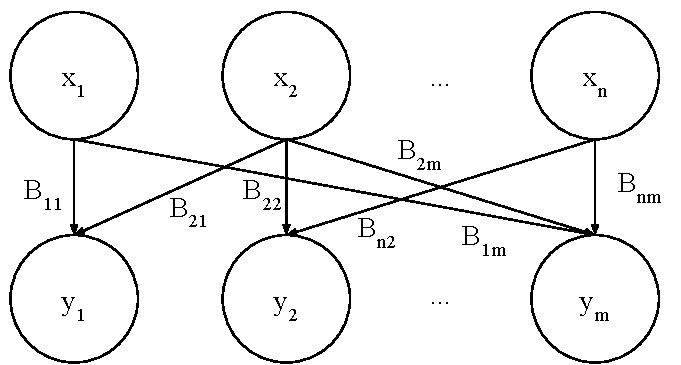
\includegraphics[width=0.75\textwidth]{hiddenmarkovmodel-2.pdf}
	\caption[Observable output of a hidden Markov model.]{Observable output of a hidden Markov model. Each state has a corresponding probability distribution for the observable outputs.}
	\label{fig:hmm-2}
\end{figure}

% Mention the joint probability distribution and cite that it also meets the markov property.
% That will be very helpful later I think.
A model where the state is a combination of $X$ and $Y$ from a \ac{HMM} is also a Markov model.
The state space for the new model, $Z$, is a set of tuples $Z = \{(X_0,Y_0), (X_0, Y_1), ... (X_1, Y_0), ... (X_n,Y_m)  \}$.
Where $\Pr(Z_k+1=(x_{k+1}, y_{k+1})|Z_k=(x_k, y_k)) = \Pr(Y_{k+1}=y_{k+1}|X_{k+1}=x_{k+1})\Pr(X_{k+1}=x_{k+1}|X_{k}=x_k)$.
Stated plainly, the probability that the joint model is some state $(x_{k+1},y_{k+1})$ is the probability that the hidden part of the model transitions to state $x_{k+1}$ and the observation for $x_{k+1}$ is $y_{k+1}$.
The probability distribution for the transition to the next state does not depend on the $y_k$ of the current state.

\section{Information Flow}

\subsection{Modal Logic}

A Kripke frame is a pair $<W,R>$\cite{french2006} such that $W$ is a set of possible worlds, where each world corresponds to a unique global state of the system.
Each element of $R$ describes a binary relationship for how the described system can move from world to world as events occur in the described system.
\nomenclature{$W$}{Set of worlds for a Kripke model or frame.}
\nomenclature{$R$}{Set of relations between worlds in a Kripke model or frame.}

In the case of a distributed system, a world could be described as one of the possible combinations of values of all boolean state variables $S=\{s_0, s_1, ... s_n\}$ in the system.
As execution occurs, messages, time, or events cause these variables to change.
Each change in boolean variables corresponds to a relationship in $R$\cite{Gehrke200565}.
Therefore, a world $w$ is one possible valuation of all the variables in $S$ and a transition from $w$ to another $w'$ (with its own valuation) can be noted as $wRw'$.
Without loss of generality, each relationship in $R$ must result in the change of at least one variable in $S$.
Additionally, the set of worlds is complete: every possible combination of state variable values is represented in the set of worlds.
No relationship in $R$ can lead to a world that does not exist.
\nomenclature{$S$}{Set of boolean state variables for a Kripke model.}

Additionally, we can define a set of valuation functions, $\mathbb{V}$.
Each function $V^i_{s_x}(w) \in \mathbb{V}$ describes the value observed by in a domain $D_i$ of a boolean state variable $s_x$ in some world $w$. 
If a valuation function for a particular state variable is not defined for an agent, the agent cannot determine the value of the state variable, and cannot determine the value of any logical statement based on the variable.
In the case of a distributed system, the valuation function concept is analogous to the isolation of memory for each agent.
For example, an agent $i$, cannot simply determine the value of a variable for agent $j$.
\nomenclature{$D_i$}{The domain of an agent or process $i$.}
\nomenclature{$\mathbb{V}$}{Set of valuation functions in a Kripke model.}
\nomenclature{$V$}{A valuation function.}

The combination of a Kripke Frame $< W,R >$ and a set of valuation functions $V$ is a Kripke model $K = \{W, R, V\}$, frequently known as a modal model.
The complete model describes all the possible worlds, the relation between those worlds and the information available in the domains of the system.
\nomenclature{$K$}{A Kripke model.}

Let $\varphi \in \Phi_0$ be an atomic proposition in a set of countably many propositions.
The set of well-formed formulas (wffs), as defined by the formulation rules in \ref{tab:axiomatic}, is the least set containing $\Phi_0$.
Additionally, we use the modal operator $\Box$ as an abbreviation for $\neg \Diamond \neg \varphi$.
The complete axiomatic system is outlined in \ref{tab:wffs}.
For the uninitiated, the modal box operator ($\Box$), ``it is necessary that'' states (in the case of $\Box \varphi$) ``in every world $w$, $\varphi$ is true.'' As its dual, the diamond operator ($\Diamond$) states ``there is a world where $\varphi$ is true.''
\nomenclature{$\varphi, \gamma, \psi$}{Well formed formulas.}
\nomenclature{$\Box \varphi$}{The modal ``it is necessary that'' operator.}
\nomenclature{$\Diamond \varphi$}{The modal ``it is possible that'' operator.}

\begin{table}[]
\small
\centering
\caption{Logical Statement Formulation Rules}
\begin{tabular}{r l}
1. & if $\varphi$ is a wff, so are $\neg \varphi$, $\Box \varphi$, and $\Diamond \varphi$. \\
2. & if $\varphi$ is a wff, so are $B_i \varphi$ and $\neg B_i \varphi$ \\
3. & if $\varphi$ is a wff, so are $T_{i,j} \varphi$ and $\neg T_{i,j} \varphi$ \\
4. & if $\varphi$ is a wff, so are $I_{i,j} \varphi$ and $\neg I_{i,j} \varphi$ \\
5. & if $\varphi$ and $\psi$ are both wff, so are $\varphi \wedge \psi$ \\
6. & if $\varphi$ and $\psi$ are both wff, so are $\varphi \vee \psi$ \\
\end{tabular}
\label{tab:wffs}
\end{table}

\begin{table}[!t]
\small
\centering
\caption{The Axiomatic System}
Definition of logical and modal operators (abbreviations) \\
\begin{tabular}{r l}
D1. & $\varphi \wedge \psi \equiv \neg ( \neg \varphi \vee \neg \psi)$\\
D2. & $\varphi \oplus \psi \equiv (\varphi \vee \psi) \wedge \neg(\varphi \wedge \psi)$ (exclusive or)\\
D3. & $\varphi \rightarrow \psi \equiv \neg \varphi \vee \psi $\\
D4. & $\varphi \leftrightarrow \psi \equiv (\varphi \rightarrow \psi) \wedge (\psi \rightarrow \varphi)$\\
D5. & $\Diamond \psi \equiv \exists w \in W : w \vdash \varphi $\\
D6. & $\Box \varphi \equiv \neg \Diamond \neg \varphi $\\
D7. & $B_i \varphi$ agent $i$ believes the truth of $\varphi$\\
D8. & $I_{i,j} \varphi$ agent $j$ informs $i$ that $\varphi \equiv \top$\\
D9. & $T_{i,j} \varphi$ agent $i$ trusts the report from $j$ about $\varphi$ \\
\end{tabular} \\~\\
Axioms \\
\begin{tabular}{r l}
P. & All the tautologies from the propositional calculus.\\
K. & $\Box (\varphi \rightarrow \psi) \rightarrow (\Box \varphi \rightarrow \Box \psi)$\\
M. & $\Box \varphi \rightarrow \varphi$\\
A1. & $\neg \Box \varphi \rightarrow \Box \neg \Box \varphi $\\
A2. & $\Diamond (\varphi \vee \psi) \rightarrow \Diamond \varphi \vee \Diamond \psi $\\
A3. & $\Box \varphi \wedge \Box \psi \rightarrow \Box (\varphi \wedge \psi)$ \\
B1. & $(B_i \varphi \wedge B_i (\varphi \rightarrow \psi )) \rightarrow B_i \psi$ \\
B2. & $\neg B_i \bot$\\
B3. & $B_i \varphi \rightarrow B_i B_i \varphi$ \\
B4. & $\neg B_i \varphi \rightarrow B_i \neg B_i \varphi$\\
I1. & $(I_{i,j} \varphi \wedge I_{i,j} (\varphi \rightarrow \psi )) \rightarrow I_{i,j} \psi$\\
I2. & $\neg I_{i,j} \bot$ \\
C1. & ($B_i I_{i,j} \varphi \wedge T_{i,j} \varphi) \rightarrow B_i \varphi$ \\
C2. & $T_{i,j} \varphi \equiv B_i T_{i,j} \varphi$ \\
\end{tabular} \\~\\
Rules of Inference \\
\begin{tabular}{r l}
R1. & From $\vdash \varphi$ and $\vdash \varphi \rightarrow \psi$ infer $\psi$ (Modus Ponens) \\
R2. & $\neg (\varphi \wedge \psi) \equiv (\neg \varphi \vee \neg \psi)$ (DeMorgan's)\\
R3. & From $\vdash \varphi$ infer $\vdash \Box \varphi$ (Generalization)\\
R4. & From $\vdash \varphi \equiv \psi$ infer $\vdash \Box \varphi \equiv \Box \psi$\\
R5. & From $\vdash \varphi \equiv \psi$ infer $\vdash T_{i,j} \varphi \equiv T_{i,j} \psi$\\
\end{tabular} \\
\label{tab:axiomatic}
\end{table}

\subsection{Non-Deducible (MSDND) Security}

In the domain of security, there are a wide variety of aspects worth protecting in every system.
These are grouped into the core security concepts of integrity, accessibility, and privacy.
Many traditional security approaches rely heavily on cryptography to provide privacy.
However, accidental information leakage can still occur, which compromises the privacy of the system.
For \ac{CPS}, the leakage is difficult to prevent.
Unlike their purely cyber counterparts, the actions taken by the physical components cannot be easily hidden from an observer.
For example, a plane changing altitude or a car turning or changing speed cannot be hidden from an observer.
Other, more complicated systems, like the power grid, have actions that are more difficult to observe. However, a well-motivated attacker can potentially collect critical information about the behavior of the cyber components with observations of the physical network\cite{Roth2012}.

Information flow security models are invaluable for assessing what information, if any, is leaked by either the cyber of physical components of the \ac{CPS}.
Many information flow security models, have been proposed, all based on similar concepts.
Typically, the models partition the system into two domains: the high-security domain and the low-security domain.
However, the MSDND security model allows the system to be partitioned into any number of domains.
The MSDND model has been used to describe how the STUXNET attack was able to hide its malicious behavior from the plant operators.
The MSDND security model is expressed using modal logic to determine what information in a domain is deducible to an observer in another domain.
The model exploits the possible worlds of modal logic to determine if there are worlds where the value of a logical atom is deducible by an agent outside the domain.

The MSDND security model can be used to determine what an agent in a distributed system can determine about another agent.
The exact specification of timing the distributed system becomes unnecessary as the modal model can express any combination of logical atoms in one of its worlds.\cite{Howser2012}\cite{STUXNET}\cite{Howser2013}

The MSDND security model can be expressed as follows\cite{STUXNET}.
Consider a pair of state variables $s_x$ and $s_y$ which may or may not be in the same security domain.
The value of $s_x$ and $s_y$ have a logical xor relationship: if $s_x$ is true, $s_y$ must be false.
Given an agent $i$ that does not have a valuation function for either of those two variables, the system is MSDND secure for the agent and pair of variables.
Written formally:

\begin{align}
MSDND = \exists w \in W : w \vdash \Box [ (s_x \vee s_y) \wedge \neg(s_x \wedge s_y) ] 
\nonumber \\ \wedge [ w \vDash ( \not \exists V_x^i (w) \wedge \not \exists V_y^i (w) ) ]
\end{align}

Of particular interest is the special case where $s_x$ and $s_y$ are relation on the same wff: $(s_x = \varphi$ and $s_y = \neg \varphi)$:

\begin{align}
MSDND = \exists w \in W : w \vdash \Box [ \varphi \oplus \neg \varphi ] 
\nonumber \\ \wedge [ w \vDash ( \not \exists V_\varphi^i(w)) ]
\end{align}

In a system where the above logical relationship holds, the agent $i$ cannot determine the value of $s_x$ or $s_y$. However, if the relationship does not hold, there is some world where the agent can determine the value of $s_x$ and $s_y$.

\subsection{BIT Logic}

% NEED CITATIONS FOR BIT LOGIC

\ac{BIT} was developed to formalize logic about belief and information transfer.
\ac{BIT} logic has typically been applied to distributed systems but has also played roles in \ac{CPS} security.
The operations of the \ac{BIT} logic allow formal definition of how entities pass information, and how they will act on the information passed to them.
\ac{BIT} logic utilizes several modal operators:

\begin{itemize}
\item $I_{i,j} \varphi$ defines the transfer of information directly from agent $j$ to an agent $i$. 
\item $T_{i,j} \varphi$ defines trust an agent $i$ has in a report from $j$ that $\varphi$ is true.
\item $B_i \varphi$ defines the belief that an agent $i$ has about $\varphi$. The actual value of $\varphi$ is irrelevant: the agent $i$ believes it to be true.
\end{itemize}
\nomenclature{$I_{i,j}$}{The modal information transfer operator.}
\nomenclature{$T_{i,j}$}{The modal trust operator.}
\nomenclature{$B_i$}{The modal belief operator.}

These operators allow reasoning about information transfer between entities.
In the context of a distributed system, these operators allow the division of the actual state held by some agent $i$ to what some other agent $j$ believes is agent $i$'s state.

\section{Explicit Congestion Notification}

\ac{ECN} is a technique for managing congestion in IP networks. 
When an \ac{ECN} capable network device detects congestion, it can drop the packets, or it can signal senders using flags in the packet headers that the network is congested.
For a TCP application, the result of the dropped packets causes the slow-start congestion control strategy to reduce the rate packets are sent.
A more advanced implementation, using \ac{ECN}, sets specific bits in the TCP header to indicate congestion.
By using \ac{ECN}, TCP connections can reduce their transmission rate without re-transmitting packets.

UDP applications have not typically utilized \ac{ECN}.
Although the \ac{ECN} standard has flags in the IPv4 header, access to the IPv4 header is not possible on most systems.
Furthermore, there is not a ``one size fits all'' solution to congestion in UDP algorithms.

\subsection{Random Early Detection (RED)}
The \ac{RED} queuing algorithm is a popular queuing algorithm for switches and routers.
It uses a probabilistic model and an \ac{EWMA} to determine if the average queue size exceeds predefined values.
The values are used to identify potential congestion and manage it.
Congestion identification is accomplished by determining the average size of the queue, and then probabilistically dropping packets to maintain the size of the queue.
In \ac{RED}, when the average queue size, $avg$, exceeds a minimum threshold ($min_{th}$), but is less than a maximum threshold ($max_{th}$), new packets arriving at the queue may be ``marked''.
The probability a packet is marked is based on the following relation between $p_{b}$ and $p_{a}$ where $p_{a}$ is the final probability a packet will be marked.

\begin{equation}
p_{b} = max_p (avg - min_{th}) / (max_{th}-min_{th})
\end{equation}
\begin{equation}
p_{a} = p_{b} / (1-count * p_b)
\end{equation}

Where $max_p$ is the maximum probability a packet will be marked when the queue size is between $min_{th}$ and $max_{th}$ and $count$ is the number of packets since the last marked packet.
With \ac{RED}, the probability a packet is marked varies linearly with the average queue size, and as a function of the time since the last packet was marked.
If $avg$ is greater than $max_{th}$, the probability of marking trends toward one as the average queue size approaches $2*max_{th}$.
In the event the queue fills completely, the \ac{RED} queue operates as a drop-tail queue.
In a simple implementation of the \ac{RED} algorithm, marked packets are dropped.

\section{Distributed Grid Intelligence (DGI)}

The DGI is a smart grid operating system that organizes and coordinates power electronics.
It also negotiates contracts to deliver power to devices and regions that cannot effectively facilitate their needs.
DGI leverages common distributed algorithms to control the power grid, making it an attractive target for modeling a distributed system.
Algorithms employed by the \ac{DGI} and grouped into modules, work together to migrate power from areas of excess supply to excess demand.

DGI utilizes several modules to manage a distributed smart-grid system.
Group management, which is our main focus, implements a leader election algorithm to discover which processes are reachable within the cyber domain.
Other modules provide additional functionality, such as collecting global snapshots, negotiating the migrations, and giving commands to physical components.

DGI is a real-time system; certain actions (and reactions) involving power system components need to be completed within a pre-specified time frame to keep the system stable.
It uses a round robin schedule where each module is given a predetermined window of execution which it may use to perform its duties.
When a module's round ends, the next module in the line is allowed to execute. 

The DGI uses the leader election algorithm, ``Invitation Election Algorithm,'' written by Garcia-Molina\cite{INVITATIONELECTION}.
The algorithm provides a robust election procedure which allows for transient partitions.
Transient partitions are formed when a faulty link inside a group of processes causes the group to divide temporarily.
The transient partitions merge when the link becomes more reliable.

\subsection{Real Time}
Real-time requirements were designed to enforce a tight upper bound on the amount of time used creating groups, discovering peers, collecting the global state, and performing migrations.

To enforce these bounds, the real-time DGI has distinct phases which modules were allowed to use for all processing.
Each module was given a round with a specific amount of processor time allocated to the module.
Modules used the allocated time to complete any tasks they had prepared.
When the allotted time was up, the scheduler changed context to the next module.
This interaction is illustrated in Figure \ref{fig:REALTIMESCHEDULER}

\begin{figure}[!h]
\centering
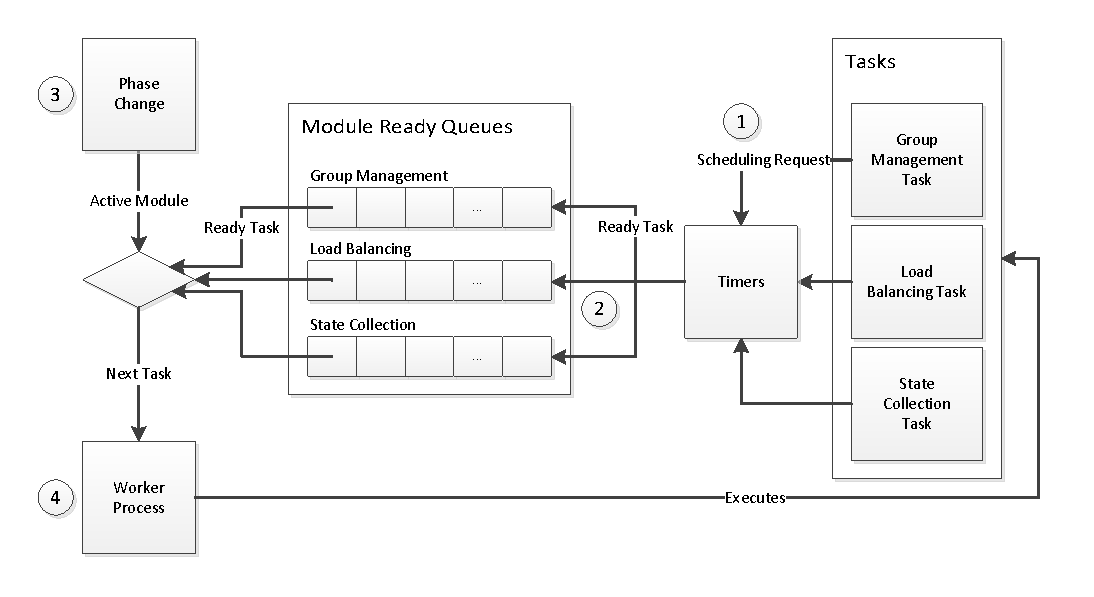
\includegraphics[width=1.0\textwidth]{RealTimeScheduler.pdf}
\captionsetup{singlelinecheck=off}
\caption[Real Time Scheduler]{The real time scheduler used a round robin approach to allot execution time to modules. 
\begin{enumerate}
    \item Modules requested a task be executed by specifying a time in the future to execute the task.
          A timer was set to count down to the specified moment.
           Modules could place tasks immediately into the ready queue if the task could be executed immediately.
    \item When the timer expires, the task is placed into the ready queue.
    \item Modules were assigned periods of execution (called phases) of a predetermined length.
          After the specified amount of time had passed, the module's phase ends and the next module in the schedule began to execute.
    \item The worker selected the next ready task for the active module from the ready queue and executed it.
          These tasks could also schedule other tasks to be run in the future.
\end{enumerate}
}
\label{fig:REALTIMESCHEDULER}
\end{figure}

Modules informed the scheduler of tasks they wish to perform.
The tasks could be scheduled for some point in the future, or scheduled to be executed immediately.
When a task became ready, it was inserted into a ready queue for the module which scheduled the task.

When the module's phase was active, tasks were pulled from the ready queue and executed.
When the phase was complete, the scheduler stopped pulling tasks from the previous module's queue and began pulling from the next module's queue.

Using a round robin scheduler allowed enforcement of an upper bound on message delay.
Modules had a specific amount of processing time allotted.
Modules with messages that invoked responses typically required the responses to be received within the same phase.
Round numbers enforced that the message was sent within the same phase.

Modules were designed and allotted time to allow for parameters such as maximum query/response time (based on the latency between communicating processes).
Modules using the scheduler had an upper-bound in response time before messages were considered lost.

\subsection{Group Management Algorithm}

The DGI uses the leader election algorithm, ``Invitation Election Algorithm,'' written by Garcia-Molina\cite{INVITATIONELECTION}.
Originally published in 1982, the algorithm provides a robust election procedure that allows for transient partitions.
Transient partitions are formed when a faulty link between two or more clusters of \ac{DGI} causes the groups to divide temporarily.
These transient partitions merge when the link becomes more reliable.
The election algorithm allows for failures that disconnect two distinct sub-networks.
These sub-networks are fully connected, but connectivity between the two sub-networks is limited by an unreliable link.

Since Garcia-Molina's original publication \cite{INVITATIONELECTION}, a large number of election algorithms have been created. 
Each algorithm is designed to be well-suited the problem space where it is used.
Specialized algorithms exist for wireless sensor networks\cite{LE-WSN-1}\cite{LE-WSN-2}, detecting failures in certain circumstances\cite{LE-SPECIALCIRCUMSTANCES-1}\cite{LE-SPECIALCIRCUMSTANCES-2}, and of course, transient partitions.
Work on leader elections has been incorporated into a variety of distributed frameworks: Isis\cite{ISISTOOLKIT}, Horus\cite{HORUSTOOLKIT}, Totem\cite{TOTEMTOOLKIT}, Transis\cite{TRANSISTOOLKIT}, and Spread\cite{SPREADTOOLKIT} all have methods for creating groups.
Despite the broad range of work, the fundamentals of leader election are consistent
across all work.
Processes arrive at a consensus of a single peer that coordinates the group.
Processes that fail are detected and removed from the group. 

The elected leader is responsible for making work assignments, and identifying and merging with other coordinators when they are found, as well as maintaining an up-to-date list of peers for the members of his group. 
Group members monitor the group leader by periodically checking if the group leader is still alive by sending a message. 
If the leader fails to respond, the querying nodes will enter a recovery state and operate alone until
they can identify another coordinator.
Therefore, a leader and each of the members maintains a set of processes which are currently reachable, a subset of all known processes in the system.

Leader election can also be classified as a failure detector\cite{LEADERELECTIONEVAL}.
Failure detectors are algorithms which detect the failure of processes within a system; they maintain a list of processes that they suspect have crashed.
This informal description gives the failure detector strong ties to the leader election process. 
The group management module maintains a list of suspected processes which can be determined from the set of all processes and the current membership.

The leader and the members have separate roles to play in the failure detection process.
Leaders use a periodic search to locate other leaders to merge groups.
This query also serves to detect failures within the system.
The member sends a query to its leader.
The member will only suspect the leader and not the other processes in their group.

Using a leader election algorithm allows the \ac{FREEDM} system to autonomously reconfigure in the event of a failure.
Cyber components are tightly coupled with the physical components, and reaction to faults is not limited to faults originating in the cyber domain.
Processes automatically react to crash-stop failures, network issues, and power system faults.
The automatic reconfiguration allows processes to react immediately to issues, faster than a human operator, without relying on a central configuration point.
However, it is important the configuration a leader election algorithm supplies is one where the system can do viable work without causing physical faults like voltage collapse or blackouts\cite{HARINI}.

A state machine for the election portion of the election algorithm is shown in Figure \ref{fig:statemachine}.
In the normal state, the election algorithm regularly searches for other coordinators.
When another coordinator is identified, all other processes will yield to their future coordinator.
The method of selecting which process becomes the coordinator of the new group differentiates the modified algorithm from other approaches.

\subsection{Power Management}

We utilized the load balancing algorithm from \cite{LOADBALANCING}.
The load balancing algorithm performs work by managing power devices with a sequence of migrations\cite{HILTESTBED}.
In each migration, a sequence of message exchanges identify processes whose power devices are not sufficient to meet their local demand and other processes supply them with power by utilizing a shared bus.
First, processes that cannot meet their demand announce their need to all other processes.
Processes with devices that exceed their demand offer their power to processes that announced their need.
These processes perform a three-way handshake.
At the end of the handshake, the two processes have issued commands to their attached devices to supply power from the shared bus and to draw power from the shared bus.
An example of how the power system is affected by migrations is depicted in Figure \ref{fig:good-migrations}.
In the chart, processes with net generation (generation $>$ 0) share power with processes with excess loads.
As processes with excess loads are satisfied, both supply and demand processes trend toward 0 net generation.

\begin{figure}
\centering
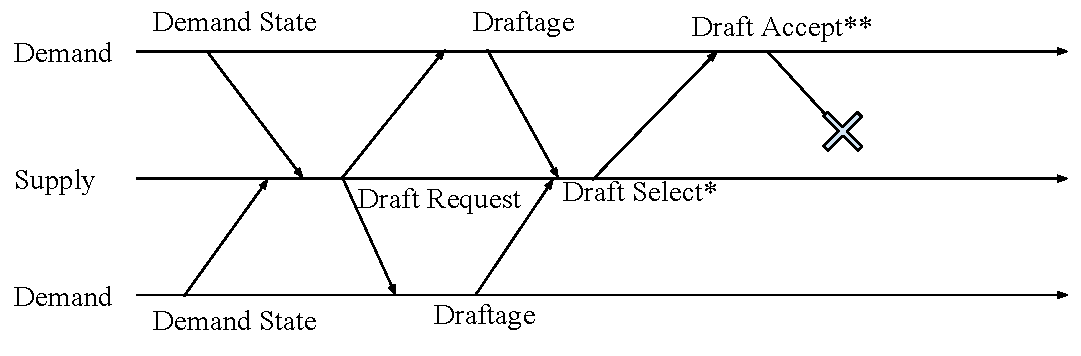
\includegraphics[width=0.95\textwidth]{FailedMigration1}
\caption{Example of a failed migration. (*) and (**) mark moments when power devices change state to complete the physical component of the migration. In this scenario, the message confirming the demand side made the physical is lost, leaving the supply node uncertain.}
\label{fig:failed-migration-1}
\end{figure}

\begin{figure}
\centering
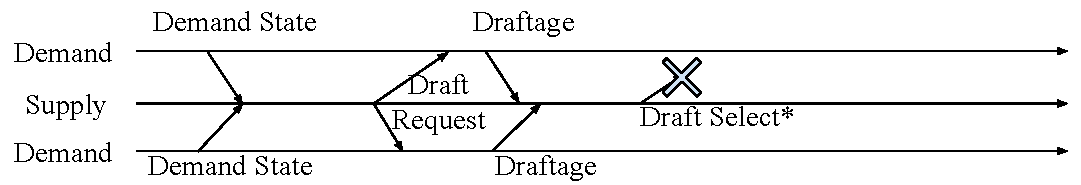
\includegraphics[width=0.95\textwidth]{FailedMigration2}
\caption{Example of a failed migration. (*) marks a moment when power devices change state to complete the physical component of the migration. In this scenario, the supply process changes its device state, but the demand process does not.}
\label{fig:failed-migration-2}
\end{figure}

\begin{figure}
\centering
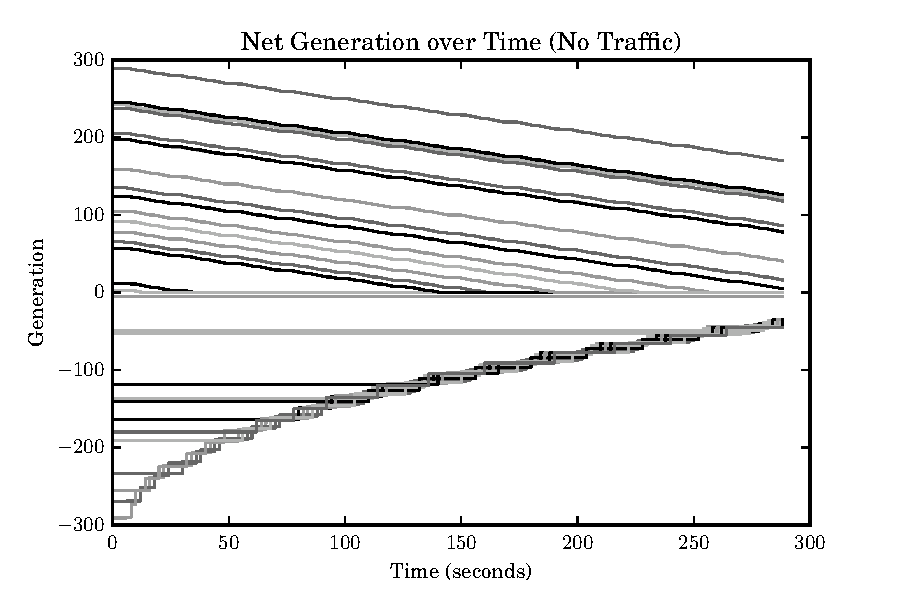
\includegraphics[width=0.75\textwidth]{c-migrations-no-traffic-all}
\caption{Each migration consumes excess generation capability and removes excess demand.}
\label{fig:good-migrations}
\end{figure}

The \ac{DGI} algorithms can tolerate packet loss and is implemented using UDP to pass messages between \ac{DGI} processes.
Effects of packet loss on the \ac{DGI}'s group management module have been explored in \cite{CRITIS2012} and \cite{JOURNAL}.
The load balancing algorithm can tolerate some message loss, but lost messages can cause migrations to only partially complete, which can cause instability in the physical network.
A failed migration is diagrammed in Figures \ref{fig:failed-migration-1} and \ref{fig:failed-migration-2}.
With the power migration algorithm, uncompensated actions may occur in the power system.
These actions can eventually lead to power instability through issues such as voltage collapse.
Additionally, the supply process may not always be certain if the second half of the action was completed or not.
If the ``Draft Accept'' message does not arrive from the demand process, the supply process cannot be certain of if its ``Draft Select'' message was received.
If the supply process takes action to compensate by reversing the migration and the confirmation arrives later, the system will also be driven towards instability because another process completed an uncompensated action.
Processes could confirm the number of failed migrations with a state collection technique.
It is, therefore, desirable to manage the processes to minimize the number of failed migrations.



% APPLICATION
% - Usage Theory
%       - Instead of dropping packets, the network device with \ac{RED} will send messages to an application announcing congestion
%       - These announcements allow the \ac{CPS} to adjust its behavior to allow better operation during the network fault.
%       - Network layout and design
%       - What are the goals of the successful operation of the \ac{CPS} algorithm
%       - Balance the amount of K that accumlates, while maximizing the amount of work done.
%       - Describe the type of traffic we are accounting for
% - What happens on the receipt of a Soft \ac{ECN} Message & Motivate this approach
% - What happens on the receipt of a hard \ac{ECN} message & Motivate this approach
% - Justify why these approaches are good for the \ac{CPS}.
% - Make sure there's mathy stuff about why this is better.
% - Justification using the models developed in the last paper--
%   - The congestion would normally cause \ac{RED} to drop packets at a certain rate, we're entering a contract with the router to change behavior rather than having an omission rate.
% - Tune \ac{RED} parameters based on Journal paper?

\section{Application}
\label{sect:application}

\subsection{Usage Theory}
When the \ac{RED} algorithm identifies congestion it must notify senders of congestion.
Since the \ac{ECN} fields in IPv4 are not available to applications running on the system, the notifications are multicast onto the source interface.
Additionally, since this approach is non-standard and most UDP applications would not understand the notification, we have opted to create an application that runs on the network device.
This application is responsible for generating the multicast message.
It also keeps a register of hosts running applications that support reacting to the \ac{ECN} notification.

%There are several reasons for this approach.
%First, related work has shown an \ac{ECN} strategy without some other queue management scheme is not sufficient to prevent congestion.
%By allowing real-time applications that decrease the number of messages for congestion special priority in the \ac{RED} algorithm, we allow those applications to continue operating during congestion.
%Additionally, in later sections, we demonstrate this strategy is effective for managing congestion.

When the \ac{RED} algorithm detects congestion, it sends a multicast beacon to a group of interfaces informing of the level of congestion.
For similarity with the \ac{RED} algorithm and the \ac{NS3} implementation, this notification is classified as either ``soft'' or ``hard.''
A soft notification is an indication the congestion in the network is approaching a level where real-time processes can expect message delays that may affect their normal operation.
A hard notification indicates the congestion has reached a level where messages may be subject to both delay and loss.
The notifications are rate limited so they do not flood the network.

\subsection{Group Management}

The group management module's execution schedule is broken into several periods of message generation and response windows.
Because the schedule of the \ac{DGI} triggers the execution of group management modules approximately simultaneously, the traffic generated by modules is bursty.
The number of messages sent is $O(n^2)$ (where n is the number of processes in the system), in a brief window, which is dependent on how well the clocks are synchronized in the system.
The duration of the response window is dependent on the amount of time it takes for messages to propagate to the hardest-to-reach process the \ac{DGI} hopes to group with.
Additionally, to contend with congestion, an additional slack must be added to allow the \ac{RED} algorithm to detect congestion before it reaches a critical level.

Figure \ref{fig:queue-types} depicts typical queueing behavior for a network device serving \ac{DGI} processes under different circumstances.
Because the traffic generated by \ac{DGI} modules is very bursty, the queue experiences a phenomena where the bursty traffic mixed with a steady background traffic causes the queue to fill.
With no background traffic, the impulse queues a large number of messages, but those messages are distributed in a timely manner.
When the background traffic is introduced, the queue takes longer to empty.
At a critical threshold, the queue does not empty completely before the next burst is generated by the \ac{DGI}.
In this scenario, the queue completely fills and no messages can be distributed.
The \ac{RED} algorithm and \ac{ECN} are used to delay or prevent the queue from reaching this critical threshold.

\begin{figure}

\includegraphics[width=\linewidth]{QueueStacked}
\caption{
Example of network queueing during \ac{DGI} operation. \ac{DGI} modules are semi-synchronous, and create bursty traffic on the network.
When there is no other traffic on the network (solid line), the bursty traffic causes a large number of packets to queue quickly, but the queue empties at a similar rate.
With background traffic (dashed line), the bursty traffic causes a large number of packets to be queued suddenly. More packets arrive continuously, causing the queue to drain off more slowly.
When the background traffic reaches a certain threshold (dotted line), the queue does not empty before the next burst occurs. When this happens, messages will not be delivered in time, and the queue will completely fill.
}
\label{fig:queue-types}
\end{figure}

For this work, the algorithm from \cite{JOURNALANON} was used.
This algorithm has a higher message complexity when in a group than the Garcia-Molina algorithm it is based on.
However, it does possess a desirable memoryless property that makes it easy to analyze.
This work uses an improved version of the algorithm which removes the restrictions in \cite{JOURNALANON} where only one process could become the leader.

\subsubsection{Soft \ac{ECN}}

A soft \ac{ECN} message indicates the network has reached a level of congestion where the router suspects processes will not be able to meet their real time requirements.
The soft \ac{ECN} message encourages the \ac{DGI} processes to reduce the number of messages they send to reduce the amount of congestion they contribute to the network, and to allow for reliable distribution techniques to have additional time to deliver messages (since fewer messages are being sent).
In the case of potential congestion, the group management module can reduce its traffic bursts by disabling elections during the congestion.
When the elections are disabled, messages for group management are only sent to members of the group.
Processes do not seek out better or other leaders to merge with.
As a consequence, the message complexity for processes responding to the congestion notification reduces from $O(n^2)$ to $O(n)$.

\subsubsection{Hard \ac{ECN}}

In a hard \ac{ECN} scenario, the router will have determined congestion has reached a threshold where the real-time processes will soon not be able to meet their deadlines.
In this scenario, the real-time process will likely split its group.
In an uncontrolled situation, the split will be random.
It is therefore desirable when this level of traffic is reached to split the group.
Splitting the group reduces the number of messages sent across the router for modules with $O(n^2)$ (where $n$ is the number of processes in the original group) message complexity.
For larger groups, splitting them provides a significant savings in the number of messages that must be queued by the router, especially since the traffic is very bursty.

\begin{figure}
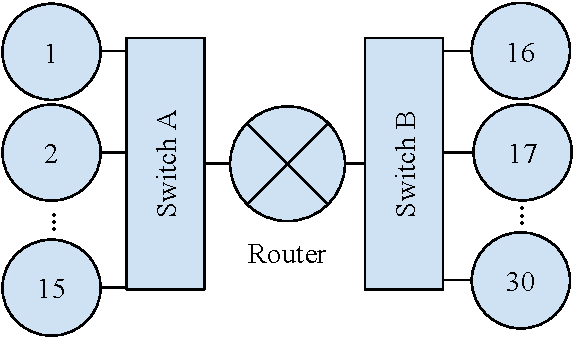
\includegraphics[width=\linewidth]{NetworkLayout}
\caption{Example of process organization used in this paper. Two groups of processes are connected by a router.} \label{fig:network-layout}
\end{figure}

Suppose a network like one depicted in Figure \ref{fig:network-layout}, where processes are divided by a router.
In Figure \ref{fig:network-layout}, there are $n$ processes on one side of the network and $m$ on the other.
In normal operation the omission-modelable algorithm has an $O(n^2)$ message complexity.
In Soft \ac{ECN} maintenance mode, the reduced number of messages reduces the complexity to $O(n)$ by disabling elections.

During elections (and with each group update) the leader distributes a fallback configuration that will coordinate the division of the groups during intense congestion.
When the \ac{ECN} notification is received the processes will halt all current group management operations and enter a splitting mode where they switch to the fallback configuration.
The leader of the group distributes a fallback notification to ensure all processes in the group apply their new configuration. 
The complexity of distributing the notification is linear $O(n)$ and processes that already received the notification will have halted their communication.
This approach will ideally avoid the burst/drain phenomena from figure \ref{fig:queue-types}.

The design of the fallback configuration can be created to optimize various factors.
These factors include cyber considerations, such as the likely network path the processes in the group will use to communicate.
By selecting the group around the network resources, the group can be selected to minimize the amount of traffic that crosses the congested links in the future.
Additionally, considerations from the physical network can be considered.
Fallback groups can be created to ensure they can continue to facilitate the needs of the members.
This can take into the consideration the distribution of supply and demand processes in the current group.
By having a good mix of process types in the fallback group the potential for work can remain high.

\subsection{Cyber-Physical System}

For a real-time \ac{CPS}, message delays could affect coordinated actions.
As result, these actions may not happen at the correct moments or at all.
Since the two-army problem prevents any process from being entirely certain a coordinated action will happen in concert, problems arising from delay or omission of messages is of particular interest.
In particular, we are interested in the scenario from \cite{HARINI}, where only half of a power migration is performed.
Other power management algorithms could have similar effects on the power system based on this idea of a process performing an action that is not compensated for by other processes.

\subsubsection{Soft \ac{ECN}}

In a soft congestion notification mode, the process being informed of the congestion can reduce its affect on the congestion by changing how often it generates bursty traffic.
Processes running the load balancing algorithm make several traffic bursts when they exchange state information and prepare migrations.
As shown before, if the interval between these bursts is not sufficient for the queue to drain before the next burst occurs, then critical, overwhelming congestion occurs.
Since the schedule of the \ac{DGI} is fixed at run-time processes cannot simply extend the duration of the load balancing execution phase.
However, on notification from the leader, the process can, instead, adjust the number of migrations to increase the message delivery interval.
This notification to reduce the schedule originates from the coordinator as part of the message exchange necessary for the process to remain in the group.
Every process in the group must receive this message to participate in load balancing, ensuring all processes remain on the same real-time schedule.
Using this approach, the amount of traffic generated is unchanged but the time period a process waits for the messages to be distributed is increased.

\subsubsection{Hard \ac{ECN}}

When the \ac{DGI} process receives a hard congestion notification, the processes switch to a predetermined fallback configuration.
This configuration creates a cyber partition.
By partitioning the network, the number of messages sent by applications with $O(n^2)$ message complexity can be reduced significantly.
Each migration of load balancing algorithm begins with an $O(n^2)$ message burst and so benefits from the reduced group size created by the partition.

Suppose there is a network like the in Figure \ref{fig:network-layout} with $n$ processes on one half and $m$ on the other.
The number of messages sent across the router for the undivided group is of the order $2mn$ as the $n$ processes on side A send a message to the $m$ on side B and vice-versa.
Let $i_{1}$ and $j_{1}$ be the number of processes from side A and side B (respectively) in the first group created by the partition.
Let $i_{2}$ and $j_{2}$ be the number of processes in the second group created by the partition under the same circumstances of $i_1$ and $j_1$.
The number of messages sent that pass through the router, is then 

\begin{equation}
2 i_{1} j_{1} + 2 i_{2} j_{2}
\end{equation}

For an arbitrary group division, the following can be observed.
Suppose $i_{1}$ and $j_{2}$ are the cardinality of two arbitrarily chosen sets of processes from side A and side B respectively.
Following the same cut requirements as before:

\begin{equation}
i_2 = n - i_1
\end{equation}
\begin{equation}
j_2 = m - j_1
\end{equation}

The the number of messages that must pass through the router for this cut is:

\begin{equation}
2 i_{1} j_{1} + 2 (n-i_{1}) (m-j_{1})
\end{equation}
\begin{equation}
= 2 i_{1} j_{1} + 2 (nm - mi_{1} - nj_{1} + i_{1}j_{1})
\end{equation}
\begin{equation}
= 2 (2 i_{1} j_{1} + nm - mi_{1} - nj_{1})
\end{equation}

The value is maximized when $i_1$ and $j_1$ are $\frac{n}{2}$ and $\frac{m}{2}$:

\begin{equation}
2( 2 \frac{mn}{4} + mn - \frac{mn}{2} - \frac{mn}{2})
\end{equation}
\begin{equation}
= mn
\end{equation}

Which is a reduction of half as many messages.
For systems with a large number of participating processes this represents a significant reduction in the number of messages sent across the router.
As a consequence, this further extends the delivery window for processes sending messages.

In the best case scenario, some cut will have a single process opposite a large number of processes.
Consider cut where one process is selected from side A and $m-1$ are selected from side B.
The cut will also create a second group of $n-1$ processes from side A and one process from side B.

\begin{equation}
2(m-1) + 2(n-1)
\end{equation}

Which represents a reduction in message complexity from the original $2mn$.

\subsection{Relation To Omission Model}

The synchronization of clocks in the environment is assumed to be normally distributed around a true time value provided by the simulation.
The shape of the curve created by plotting the queue resembles that of the \ac{CDF} of the normal distribution, noted $F(x)$.
A simple description of the traffic behavior can then be described in terms of that curve.
First, observe that when the queue hits a specific threshold, even if the queue is drained at an optimal rate, the $n$th queued packed will not be delivered in time:

\begin{equation}
Qsize - min(Qsize, (DequeueRate * \Delta t)) \geq 0
\label{eq:origin}
\end{equation}

Where $\Delta t$ is the deadline for the message to be delivered.
If the size of the queue exceeds the number of messages that can be delivered before $\Delta t$ passes, some messages will not be delivered.
The size of the queue during the message bursts created by the DGI depends on the message complexity of the algorithm, the number of messages already in the queue, the other traffic on the network, and any replies that also have to be delivered in that interval.
Therefore, let $c$ represent the rate that traffic is generated by other processes.
Let $init_q$ represent the number of messages in the queue at the start of a burst. 
Let $init_m$ represent the number of messages sent in the beginning of the burst.
Let $resp$ represent the number of messages sent in response to the burst that must still be delivered before $\Delta t$ passes.
We can then express $Qsize$ as two parts:

\begin{equation}
Qsize = Burst + Obligations
\end{equation}

Where $Burst$ takes the form of the \ac{CDF} for the normal distribution:

\begin{equation}
Burst = init_m * F(x)  
\end{equation}

\begin{equation}
Obligations = c * \Delta t + init_q + resp
\end{equation}

From this we can derive the equation:

\begin{equation}
F(x) \geq \frac{DequeueRate * \Delta t - c * \Delta t - init_q - resp}{init_m}
\label{eq:prob-est}
\end{equation}

Where, from Equation \ref{eq:origin}, $DequeueRate * \Delta t$ is less than or equal to the number of messages in the queue. 
Solving for $F(x)$ gives a worst case estimate of the omission rate for a specific algorithmic or network circumstance.
$DequeueRate$ is affected by the amount of traffic in the system. 
It should be obvious a greater amount of background traffic corresponds to a greater average queue size.
From an relationship between the background traffic and the average queue size and the results presented in \cite{JOURNALANON}, Equation \ref{eq:prob-est} can be used to select the ECN parameters.

% EXPERIMENTAL SETUP
% - Setup
%   \ac{DGI}
%   \ac{NS3}
%   Boost
% - Describe the setup -- Network layout, \ac{DGI} placement at nodes, Random seeds?
% - Describe the quantites we are looking at? What the graphs will mean. Establish the control-- normal operation.
% - Network behavior during the experiments.

\section{Experimental Setup}

Experiments were run in a Network Simulator 3.23 test environment.
The simulation time replaced the wall clock time in the \ac{DGI} for the purpose of triggering real-time events.
As a result, the computation time on the \ac{DGI}s for processing and preparing messages was neglected.
However, to compensate for the lack of processing time, the synchronization of the \ac{DGI}s was instead distributed as a Gaussian distribution.
This was done to introduce realism to ensure that evens did not occur simultaneously as that is a physical impossibility.
Additionally, the real-time schedules used by the \ac{DGI} were adjusted to remove the processing time that was neglected in the simulation.

The \ac{DGI}s were place into a partitioned environment.
The test included 30 nodes.
Each of the nodes ran one \ac{DGI} process.
Two sets of 15 \ac{DGI} were each connect to a switch and each switch was in turn connected to the router.
This network is pictured in Figure X.
Node identifiers were randomly assigned to nodes in the simulation and used as the process identifier for the \ac{DGI}.

The links between the router and the switches had a \ac{RED} enabled queue placed on both network interfaces.
The \ac{RED} parameters for all queues were set identically.
A summary of \ac{RED} parameters are listed in Table X.
All links in the simulation were 100Mbps links with a 0.5ms delay.
RED was used in packet count mode to determine congestion.
ARP tables were populated before the simulation began.

\begin{table*}
\begin{tabular}{ | l | l | } \hline
Parameter & Value         \\ \hline
RED Queueing Mode & Packet\\ \hline 
RED Gentle Mode & True    \\ \hline
RED $Q_{w}$ & 0.002       \\ \hline
RED Wait Mode & True      \\ \hline
RED Min Threshold & 90    \\ \hline
RED Max Threshold & 130   \\ \hline
Maximum Queue Size & 1000 \\ \hline
RED Link Speed & 100 Mbps \\ \hline
RED Link Delay & 0.5 ms   \\ \hline
\end{tabular}
\caption{Summary of \ac{RED} parameters. Unspecified values default to the \ac{NS3} implementation default value}
\label{tab:red-parameters}
\end{table*}

To introduce traffic, a process attached to each of the switches attempted to send a high volume of messages to each other across the router.
Due to the bottleneck due to the properties of the network links, the greatest queueing effect occurred at the switch where the packets originated.


% RESULTS
%   - Show the unbounded Queue Graph and the mess it makes of LB and GM
%   - Show soft ECVN allows more work to be done, possibly at the cost of accumulating K.
%   - Shwo that HARD ecn allows the best operation -- work gets done and less K is accumlated.
\chapter{Conclusion}

This work presented a new approach for predicting the behavior of a real-time distributed system under omission failure conditions. By using a continuous time Markov chain, a variety of insights can be gathered about the system, including observations such as how long a particular configuration will be stable, and the behavior of the system in the long run.  The Markov results will be used  to make better real time schedules to better react to the network faults we plan on introducing to our test beds. The primary concern are scenarios in which the cyber controller attempts to make physical components which are not connected in the physical network interact, and scenarios where a fault in the cyber network causes the paired events (where two physical controllers change to accomplish some transaction or exchange) to only be partially executed. For example, in the DGI load balancing scheme, a node in a supply state injects a quantum of power into the physical network, but the node in the demand state does not change to accept it. These errors, which are the primary focus of this work could cause instability if a sufficient number of these failed exchanges occur. In \cite{HARINI}, Choudhari et. al. show that failed transactions can create a scenario where the frequency of a power system could become unstable. 

Moving forward, we have identified these areas as targets for improving the research done and creating new contributions.

\section{Time between reconfigurations}

 The rate that the system should reconfigure is a function of the maximum number of failed migrations that the system can handle before becoming unstable, the time it takes to write to the channel and the time it takes process messages. The amount of time in group can also be a consideration for which algorithm to select based on the needed amount of time to perform its work. Group Management can be used as a critical component in a real-time distributed system to manage the number of lost messages and as a consequence, the number of failed migrations in a CPS. It is critical to understand how frequently nodes enter and exit the group based on lost messages and how many migrations fail as a consequence of those messages. This area is deficient because it is strongly coupled to the interactions with the physical component: we must understand how the cyber configuration and physical changes made by that configuration can affect the system, and establish when reconfigurations should occur to keep the system stable. To correct this, we hope to develop a mathematical relationship between the stability of the group, and the physical management functionality of the CPS.

\section{Correctness of an Installed Configuration}

 The work presented in this document is probabilistic: the results of a leader election are random and based only on responses arriving with in a specified period of time. Other factors can affect what configurations can be installed such as trust in the parties in the group, the underlying physical topology, and the reliability of the peers in that group. We hope to develop guarantees on the properties of a configuration that protect the physical topology and the members of the group. These guarantees would also allow processes to better police the configurations they are installed in, in order to protect the system from malicious nodes.

\section{Accuracy of The Model}

We recognize that the model presented thus far does not have ideal accuracy. We expect to be able to further refine the model and the algorithms and formulas for generating the model. There are some features of the behavior of the DGI which are not completely encapsulated in the model. Additionally, the way models are specified can be generalized to support more systems of similar design. As part of this work however, we must remember modeling distributed systems is extremely difficult and while the increase in accuracy is desirable it is not a critical goal.

\section{Scope of the Model}

The models presented in this work focus only on the leader election component of a dynamically configured CPS. Additional work would incorporate additional components of the DGI system into the models for a more complete picture of the behavior of the system during failures. We will consider the correctness of the incorporated algorithms, how omission failures can violate that correctness, and what restrictions we can place on the configuration and operation of DGIs in order to protect the entire system during failures. To do this, we will expand the analysis performed here to incorporate algorithms such as state collection and load balancing and define metrics to quantify their behavior during omission failures. This thrust will pair with the correctness and time between reconfigurations: different algorithms will have different amounts of failure that can be allowed before reconfiguration is necessary.

\section{Deliverables}

Therefore, moving forward, we will expand the models we have presented here to include more of the properties of the complete CPS. This model will allow us to better understand what effects the group behavior has on the CPS. Using this, we can establish invariants which allow us to ensure the correctness of a CPS by providing assertions which will not be broken during execution. Creating these invariants will allow us to improve the development of CPSs, especially in their dynamic configuration, which is an area with limited development. These invariants also allow us to create an assertion of correctness which can be validated, during runtime, to ensure the system maintains its stability. We will continue to create and validate models of the CPS against simulations and actual hardware. As we do so we will construct invariants that describe the correct behavior of the groups to ensure safe operation. In addition to the existing conference paper \cite{CRITIS2012}, we have prepared a journal paper with the new work in this document. 

\subsubsection*{Acknowledgments.}

The authors acknowledge the support of the Future Renewable
Electric Energy Delivery and Management Center,
a National Science Foundation supported Engineering Research
Center under grant NSF EEC-081212, and the United States Department of Education GAANN program.

%
% ---- Bibliography ----
%
\bibliographystyle{splncs03}
\bibliography{latex_bibliography}
%


\end{document}
